%----------------------------------------------------------------------------------------
%	ANALISI DEI REQUISITI
%----------------------------------------------------------------------------------------

\section{Analisi dei requisiti}

%In questa sezione esporre brevemente i requisiti a cui il sistema proposto deve rispondere, concentrando l'attenzione sugli aspetti più rilevanti e facendo eventualmente uso di opportuni diagrammi di alto livello.\\

%  3 componenti & 8000 & 10000 \\


%

\subsection{Centralina (\textit{Control Unit})}
Ecotrip viene concretamente integrato all'interno di un albergo tramite l'installazione di apposite centraline. Come gia anticipato, queste comprendono diversi sensori cablati e dislocati all'interno delle camere. I requisiti funzionali relativi alla \textit{Control Unit} possono essere elencati in:
\begin{itemize}
    \item calcolo del consumo energetico grazie uno o più sensori di corrente;
    \item calcolo del consumo di acqua tramite due flussometri;
    \item discriminazione del flusso di acqua calda da quella fredda tramite due termostati;
    \item rilevazione dello stato delle tende (aperte/chiuse) della stanza attraverso un sensore di luminosità installato su ogni finestra;
    \item rilevazione della temperatura della stanza mediante un sensore di temperatura ambientale;
    \item rilevazione della percentuale di umidità della stanza tramite un sensore di umidità ambientale;
    \item modulo di wi-fi così da permettere alla centralina di collegarsi a Internet, mediante la rete dell'Hotel, e condividere i dati con la piattaforma in cloud;
    \item software necessario per la raccolta dei dati prodotti dai sensori e invio di un loro aggregato ogni \textit{X} secondi. Le informazioni comunicate dovranno essere riconducibili a una specifica camera di un determinato hotel;
    \item dotare la \textit{Control Unit} di un \textit{transponder} NFC  così da permettere la comunicazione tra questa e l'app Ecotrip presente nello smartphone. Nello specifico la centralina comunicherà all'app un \textit{token} con il quale l'ospite potrà richiedere alla piattaforma in cloud i dati relativi al suo pernottamento.
\end{itemize}
%
I requisiti funzionali la cui implementazione è stata ritenuta prorogabile sono:
\begin{itemize}
    \item identificazione della presenza o meno dell'ospite all'interno della stanza per promuovere l'efficacia dell'algoritmo di calcolo del punteggio. Per l'implementazione del requisito sono state definite tre possibili soluzioni:
    \begin{itemize}
        \item nel caso in cui nella camera vi sia già una centralina che controllata l'impianto elettrico tramite l'inserimento di una chiave (tessera), la presenza dell'ospite può essere rilevata dalla \textit{Control Unit} di Ecotrip reagendo all'attivazione dell'impianto;
        \item nel caso non vi sia una centralina (preesistente), la stanza dovrà dotarsi di appositi sensori installati sul soffitto e sulla porta oppure si dovrà dotare la \textit{Control Unit} di un supporto per il bluetooth. Quest'ultimo permetterà di identificare lo smartphone dell'ospite entro un raggio sufficientemente ampio da coprire l'intera stanza.
    \end{itemize}
\end{itemize}
%
Per quanto riguarda i requisiti non funzionali, questi possono essere riassunti in:
\begin{itemize}
    \item efficienza del processo di connessione tra lo smartphone dell'ospite e la centralina. Il tutto dovrà avvenire richiedendo uno sforzo minimo all'utente, si dovranno quindi evitare procedure di registrazione e/o inserimento dati. 
    \item elevato grado di UX, in particolare si dovrà porre la giusta attenzione sulla "gamification" così da veicolare efficacemente il messaggio di ecosostenibilità;
    \item sistema di monitoraggio della centralina che preveda meccanismi di controllo dello stato (centralina online/offline) e di manutenzione da remoto.
    \item buon livello di sicurezza e \textit{privacy}: le informazioni inviate all'app dovranno essere crittografate, ad esempio avvalendosi del protocollo HTTPS, ed a fronte di un check-out la centralina dovrà dissociarsi dal \textit{token}.
\end{itemize}
%
\subsection{Pannello di controllo}
Come già anticipato, le attività amministrative vengono supportate da un'apposita applicazione frontend utilizzata sia dagli amministratori di Ecotrip che dagli \textit{Hotelier}. 
I requisiti funzionali della \textit{dashboard} possono essere quindi schematizzati e suddivisi per tipologia di utente.\newline\newline
%
Funzionalità lato amministratore di Ecotrip:
\begin{itemize}
    \item gestione della lista degli hotel e delle rispettive camere registrate all'interno del sistema;
    \item visualizzazione delle centraline attualmente in uso, con eventuale gestione dei malfunzionamenti;
    \item registrazione degli account degli \textit{hotelier};
\end{itemize}
%
Funzionalità lato \textit{hotelier}:
\begin{itemize}
    \item gestione dei \textit{check-in} e \textit{check-out} degli ospiti;
    \item visualizzazione delle stanze e dei dati istantanei (consumi in tempo reale) generati dalle centraline. Per una maggiore efficacia del sistema, questa attività dovrebbe essere automatizzata integrato Ecotrip con un eventuale gestionale preesistente;
    \item visualizzazione del "punteggio sostenibilità" ottenuto da ogni ospite a fine pernottamento con relativo consumo totale di CO2. Questo permetterà di offrire all'ospite un "\textit{reward}", per esempio uno sconto. 
\end{itemize}
%
Funzionalità comuni:
\begin{itemize}
    \item meccanismo di autenticazione e autorizzazione (\textit{role-based});
    \item elevato grado di usabilità.
\end{itemize} 
%
\subsection{Applicazione}
Il coinvolgimento dell'ospite all'interno del sistema avviene tramite un'applicazione (o webapp), questa permette di sintetizzare il comportamento ed i consumi dell'utente tramite il "punteggio sostenibilità" ("gamification").\newline
%
I requisiti funzionali dell'applicazione:
\begin{itemize}
    \item connessione automatica con la piattaforma in cloud una volta ricevuto il \textit{token} dalla centralina;
    \item visualizzazione dei pernottamenti (corrente e passati) e dei dati associati come il consumo di CO2 totale e il "punteggio sostenibilità", entrambi aggiornati in tempo reale;
\end{itemize}
%
I requisiti non funzionali possono essere elencati in:
\begin{itemize}
    \item limitare il numero di dispositivi associati ad un determinato \textit{token} così da garantire un buon livello di sicurezza e privacy;
    \item UX di alta qualità.
\end{itemize}
%
\subsection*{Piattaforma in cloud}
Allo scopo di limitare i costi e ridurre i tempi di sviluppo, si è scelto di delegare diverse attività a servizi esterni. In particolare si è scelto di esternalizzare tutte le funzionalità che possono essere collocate all'interno dell'area di competenza del \textit{backend}.\newline\newline
%
In questo caso i requisiti funzionali di interesse sono:
\begin{itemize}
    \item servizio di persistenza dei dati, necessario per la memorizzazione degli utenti, dei pernottamenti (con relativi dati sintetizzati), degli hotel e delle relative stanze;
    \item meccanismo di \textit{shadowing} che permette di monitorare e gestire da remoto lo stato delle centraline. La connessione stabilita consente di comunicare alla centralina il \textit{token} che identifica il pernottamento;
    \item algoritmo di generazione dei \textit{token}, cioè codici univoci e casuali prodotti a fronte di un \textit{check-in};
    \item algoritmo per il calcolo della CO2 e del punteggio "sostenibilità"
    \begin{itemize}
        \item per effettuare il calcolo CO2 deve essere specificato per ciascun hotel il costo dell'energia nei termini di CO2/Kilowatt;
        \item il punteggio "sostenibilità" tiene conto, non solo della CO2 totale, ma anche del comportamento tenuto dall'ospite durante la sua permanenza. Alcuni atteggiamenti penalizzati possono essere l'uso eccessivo di acqua o uscire dalla camera lasciando il condizionatore accesso e le tende aperte di giorno.
    \end{itemize} 
\end{itemize}
%
I requisiti non funzionali:
\begin{itemize}
    \item scalabilità del sistema in risposta ad un notevole numero di centraline collegate;
    \item elevato livello di sicurezza.
\end{itemize}

\subsection{Casi d'uso}
Nella seguente sezione vengono presentati i casi d'uso principali suddivisi per contesto (pannello di controllo, app e centralina). Questi hanno permesso di definire i requisiti del sistema coinvolgendo attivamente il cliente, così da ricevere \textit{feedback} istantanei con cui prontamente aggiornare il diagramma. Ogni figura proposta modella una specifica parte dei requisiti poc'anzi elencati definendo inoltre gli attori interessati.

\begin{figure}[H]
    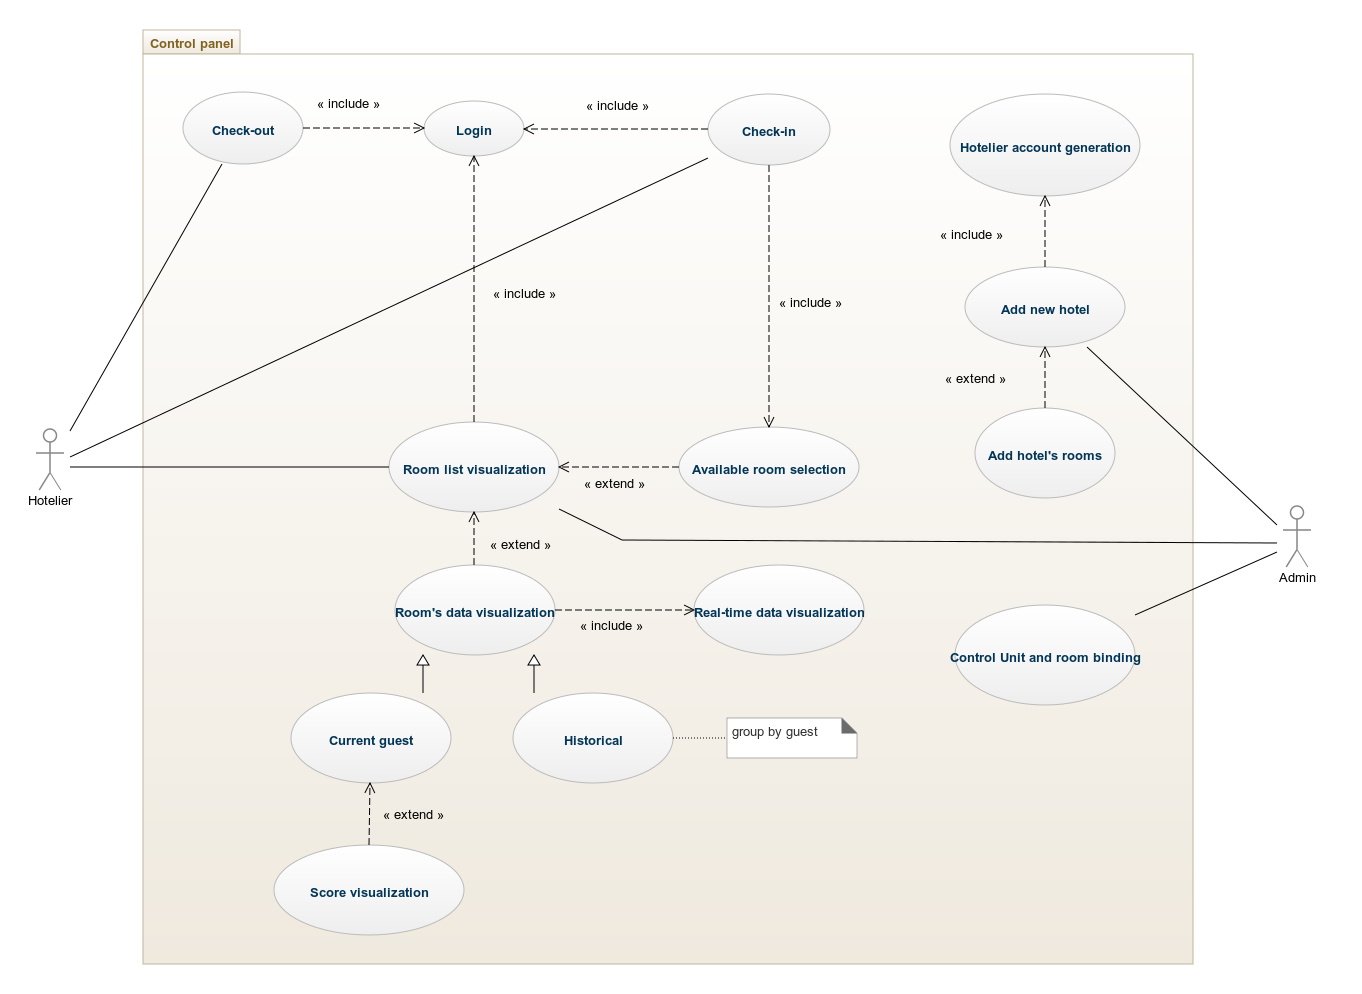
\includegraphics[width=\textwidth]{control-panel-usecase.png}
    \centering
    \caption[control-panel-usecase]{Schema dei casi d'uso del pannello di controllo.}
    \label{fig:cp-usecase}
\end{figure}

\begin{figure}[H]
    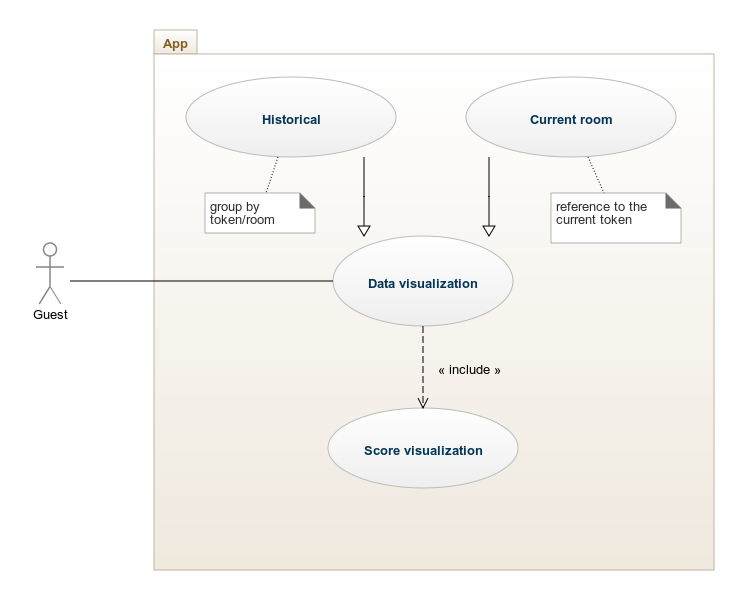
\includegraphics[width=0.8\textwidth]{app-use-case.png}
    \centering
    \caption[app-usecase]{Schema dei casi d'uso relativi all'applicazione lato ospite.}
    \label{fig:app-usecase}
\end{figure}

\begin{figure}[H]
    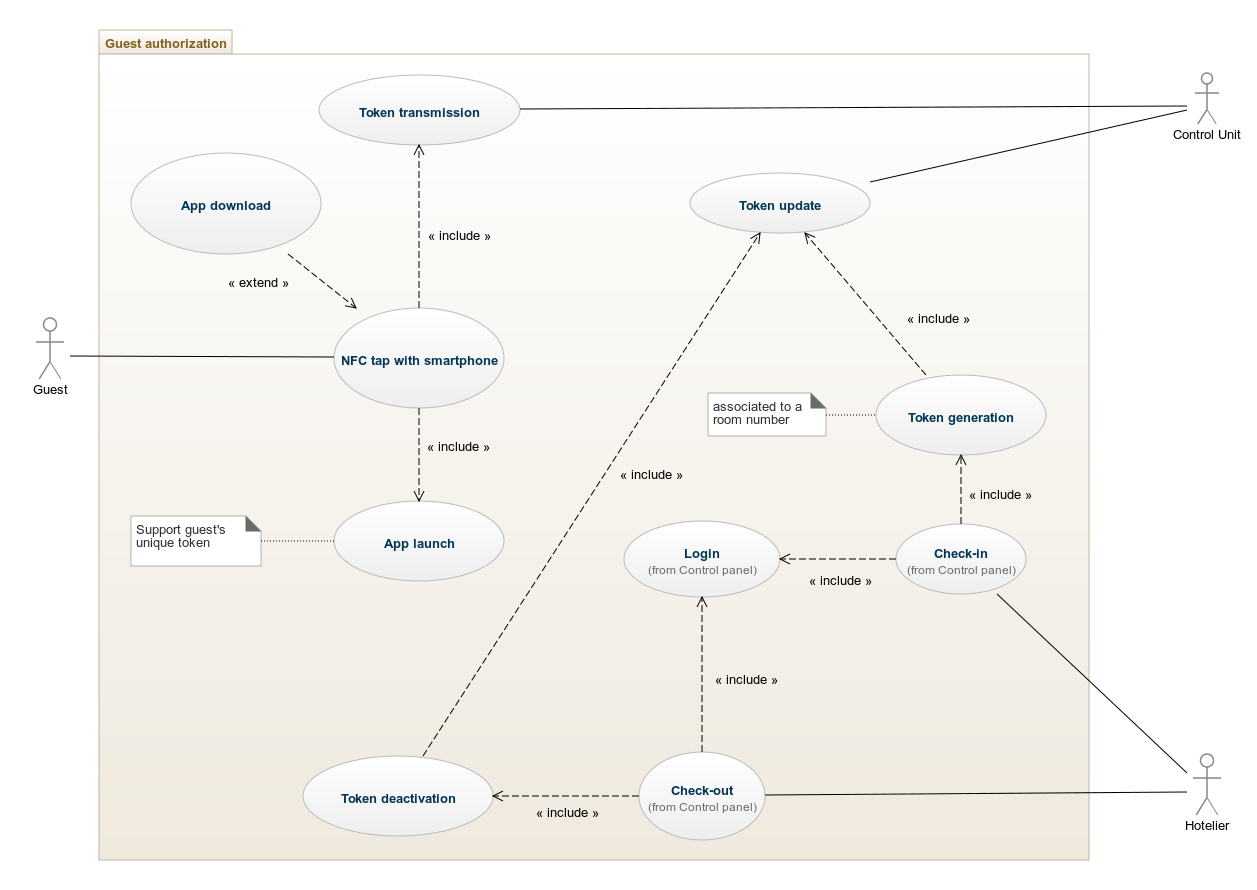
\includegraphics[width=\textwidth]{guest-authorization-use-case.png}
    \centering
    \caption[guest-authorization-usecase]{Schema dei casi d'uso del meccanismo di autorizzazione dell'ospite.}
    \label{fig:guest-authorization-usecase}
\end{figure}

\begin{figure}[H]
    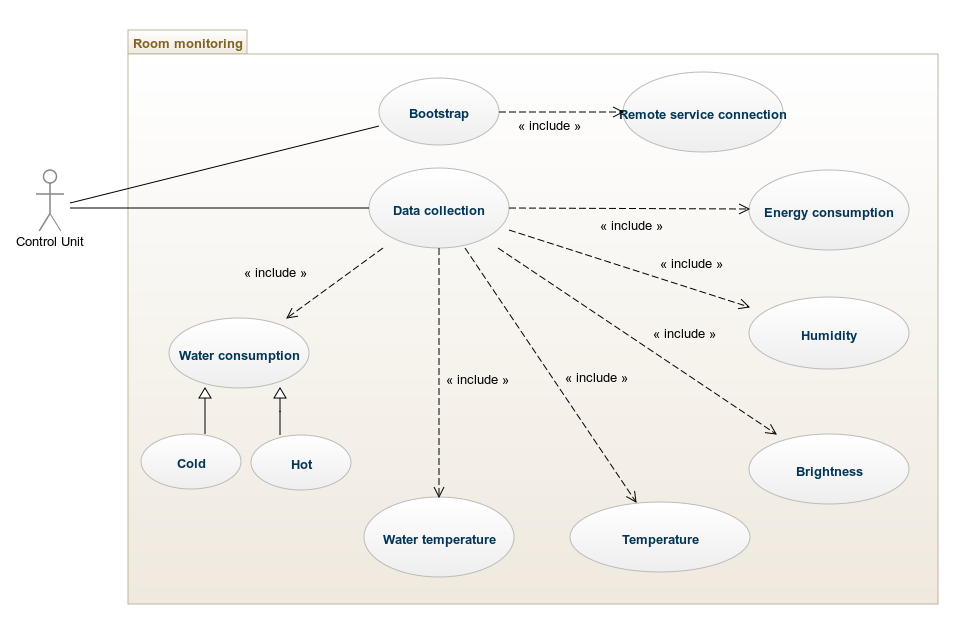
\includegraphics[width=\textwidth]{room-monitoring-use-case.png}
    \centering
    \caption[room-monitoring-usecase]{Schema dei casi d'uso relativi alla \textit{control unit}.}
    \label{fig:room-monitoring-usecase}
\end{figure}

\subsection{Identificazione dei sottodomini}
Una volta valutate le diverse responsabilità dei requisiti funzionali, precedentemente descritti, si è scelto di confinarli in 9 sottodomini (Figura \ref*{fig:subdomains}).
\begin{figure}[H]
    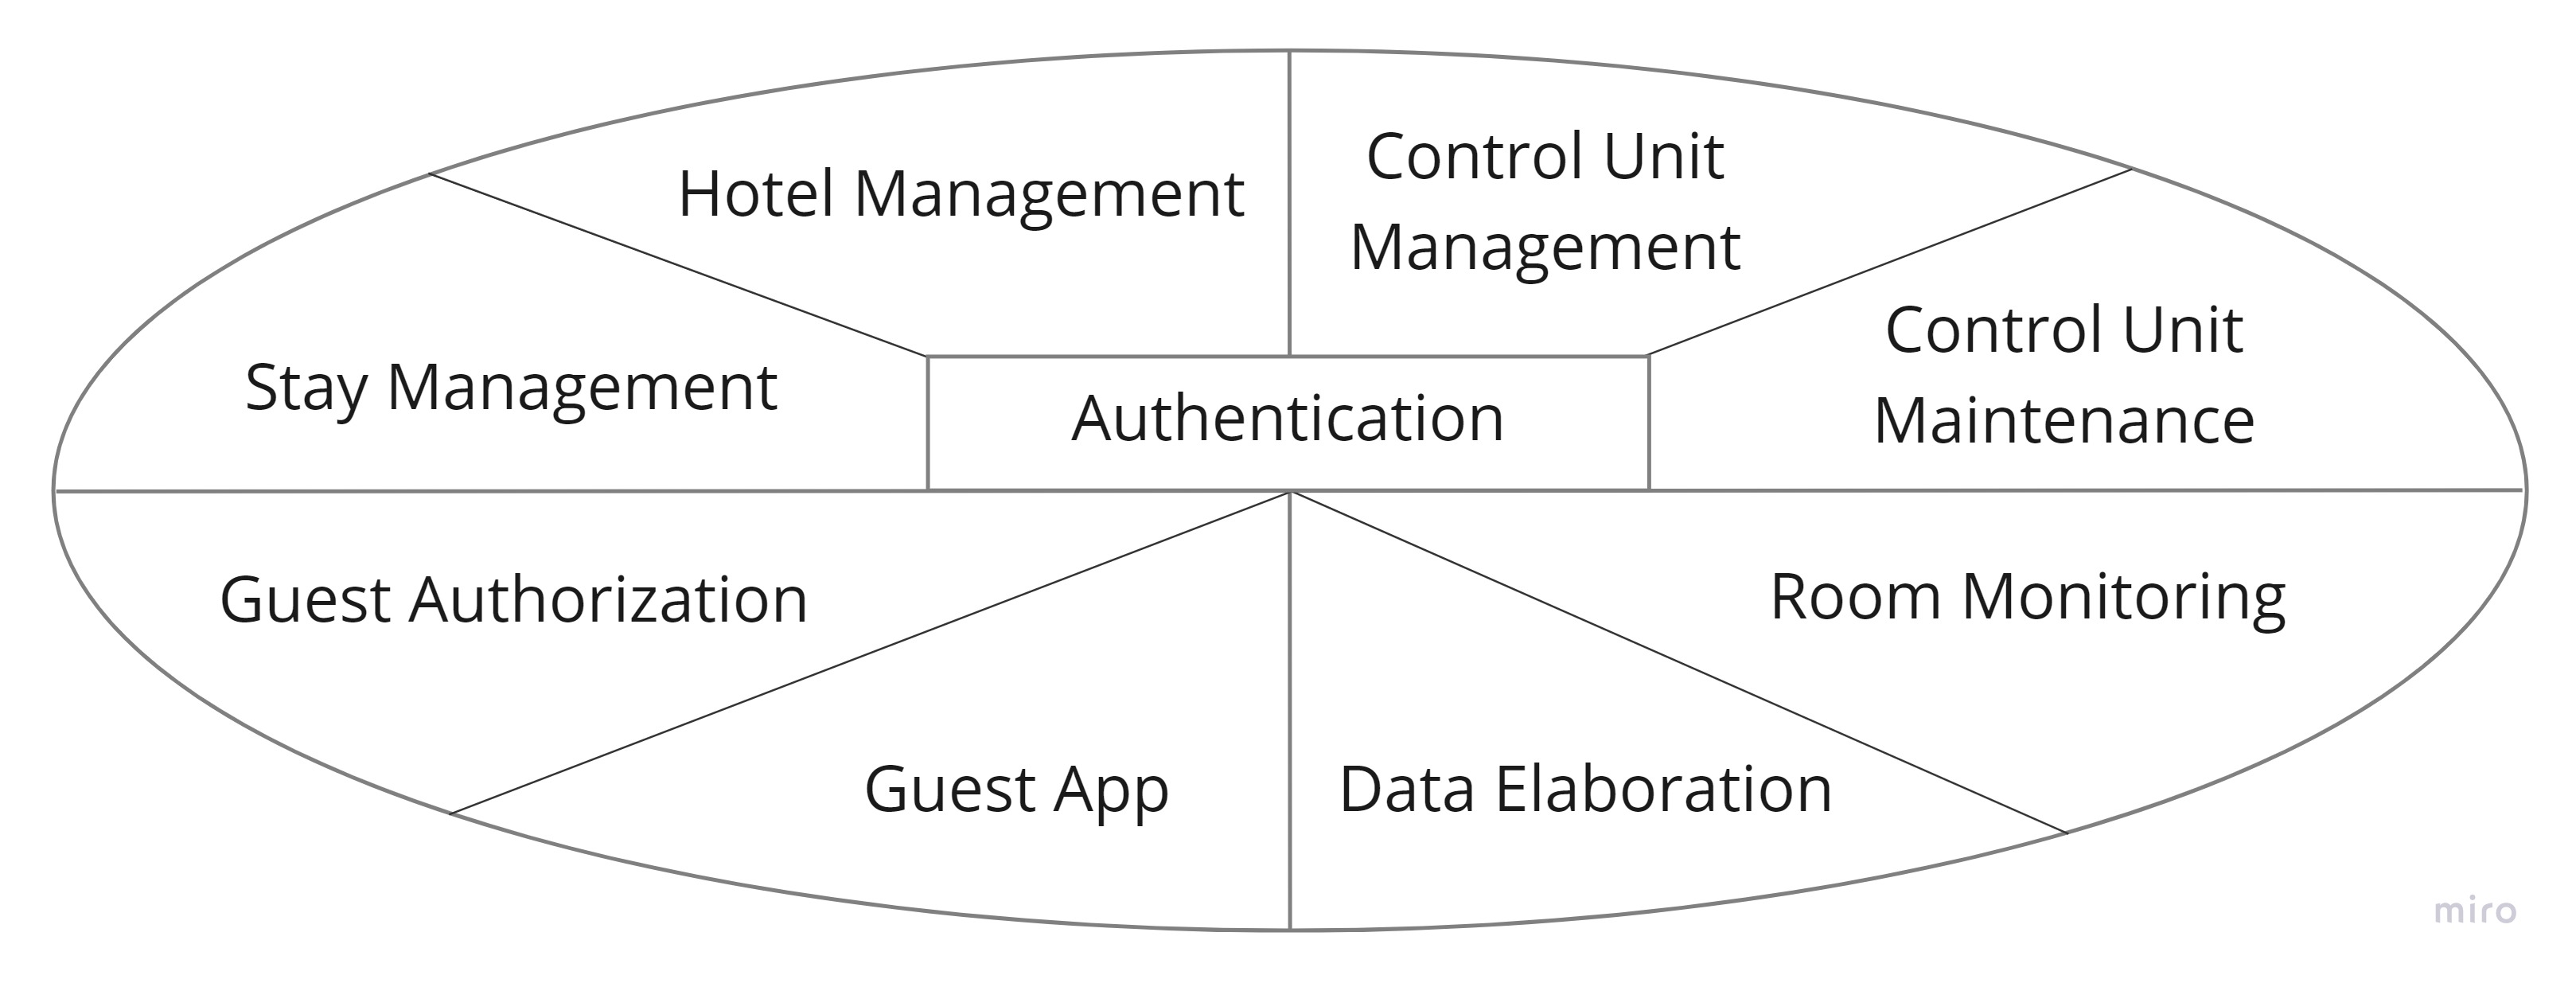
\includegraphics[width=\textwidth]{subdomains.jpg}
    \centering
    \caption[subdomains]{Sottodomini del sistema Ecotrip.}
    \label{fig:subdomains}
\end{figure}
\begin{itemize}
    \item \textit{Hotel Management}: comprende le funzionalità svolte dall'amministratore Ecotrip che riguardano la configurazione di nuovi hotel e relative camere.
    \item \textit{Stay Management}: comprende la gestione dei soggiorni con le funzioni di \textit{check-in} e \textit{check-out} da parte dell'hotelier.
    \item \textit{Authentication}: comprende sia l'autenticazione utenti quali amministratore Ecotrip e \textit{hotelier} richiesta per l'utilizzo dei servizi come \textit{Hotel} e \textit{Stay Management}, che la possibilità di registrare gli \textit{account} per gli \textit{hotelier}.
    \item \textit{Control Unit Management}: comprende la gestione delle centraline installate con la possibilità di verifica dello stato e di abbinamento alle camere.
    \item \textit{Control Unit Maintenance}: comprende il sistema per la manutenzione da remoto delle centraline installate.
    \item \textit{Room Monitoring}: comprende il sistema per il campionamento dei dati dai sensori della centralina e lo stoccaggio in un servizio cloud.
    \item \textit{Data Elaboration}: comprende il sistema per il calcolo della stima dei consumi C02 e del punteggio "sostenibilità" relativo ai soggiorni, a partire dai dati collezionati.
    \item \textit{Guest Authorization}: include il processo di generazione del \textit{token} per un nuovo soggiorno ed il suo trasferimento alla centralina e successivamente allo smartphone mediante \textit{transponder} NFC, permettendo così all'ospite di accedere ai dati del suo soggiorno.
    \item \textit{Guest App}: include la visualizzazione dei dati del soggiorno tramite applicativo fruibile dagli ospiti, inoltre implementa gli aspetti di \textit{gamification}.
\end{itemize}

\newpage